%% Figure from MATH 556 notes, section 48 (Lecture 21). ADDED (not from lecture).
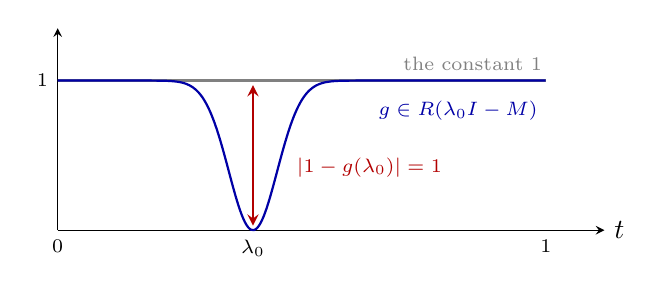
\begin{tikzpicture}[>=stealth, xscale=6.2, yscale=1.9]
    \draw[->] (0,0) -- (1.12,0) node[right] {$t$};
    \draw[->] (0,0) -- (0,1.35);
    \draw[thick, gray] (0,1) -- (1,1);
    \draw[thick, blue!65!black, domain=0:1, samples=160, smooth] plot (\x, {1 - exp(-((\x-0.4)/0.07)^2)});
    \draw[<->, thick, red!70!black] (0.4,0.03) -- (0.4,0.97);
    \node[red!70!black, font=\scriptsize, anchor=west] at (0.47,0.42) {$|1 - g(\lambda_0)| = 1$};
    \node[below, font=\scriptsize] at (0.4,0) {$\lambda_0$};
    \node[below, font=\scriptsize] at (1,0) {$1$};
    \node[below, font=\scriptsize] at (0,0) {$0$};
    \node[left, font=\scriptsize] at (0,1) {$1$};
    \node[gray, font=\scriptsize, anchor=south] at (0.85,1) {the constant $1$};
    \node[blue!65!black, font=\scriptsize, anchor=north] at (0.82,0.93) {$g \in R(\lambda_0 I - M)$};
\end{tikzpicture}
